Modify \texttt{heat\_CN.m} to produce a new m-file \texttt{heat\_trbdf2.m} which implements the TR-BDF2 method on the
same problem. Test it to confirm that it is also second-order accurate. Explain how you determined the proper boundary
conditions in each stage of the Runge-Kutta method.

\begin{solution}\ \\\\
    \hfill\vfill
    \pagebreak
    To verify second-order accuracy, we let $k = 4h$ (i.e., $\alpha = 4$); the output of \texttt{problem\_2b.m} is 
    given below:
    
    \begin{figure}[h]
        \centering
        \begin{verbatim}
                 h            k          error
            5.0000e-02   2.0000e-01   1.1471e-03
            3.3333e-02   1.3333e-01   4.8374e-04
            2.5000e-02   1.0000e-01   2.8576e-04
            2.0000e-02   8.0000e-02   1.7747e-04
            1.0000e-02   4.0000e-02   4.5852e-05
          
         Least squares fit gives E(h) = 0.43939 * h^1.99322
        \end{verbatim}
        \caption{Output of \texttt{problem\_2b.m}}
    \end{figure}

    \begin{figure*}[h]
        \centering
        \begin{subfigure}[b]{0.475\textwidth}
            \centering
            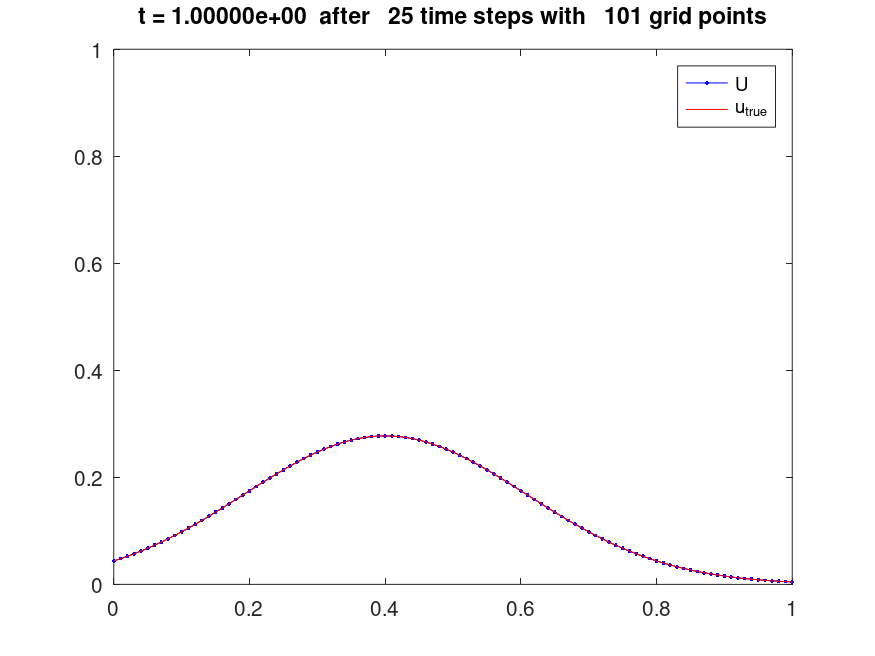
\includegraphics[width=\textwidth]{problem_2b_heatTRBDF2_t-25.png}
            \caption{TR-BDF2 method for $m = 99$ at $t = 1$}
        \end{subfigure}
        \hfill
        \begin{subfigure}[b]{0.475\textwidth}
            \centering
            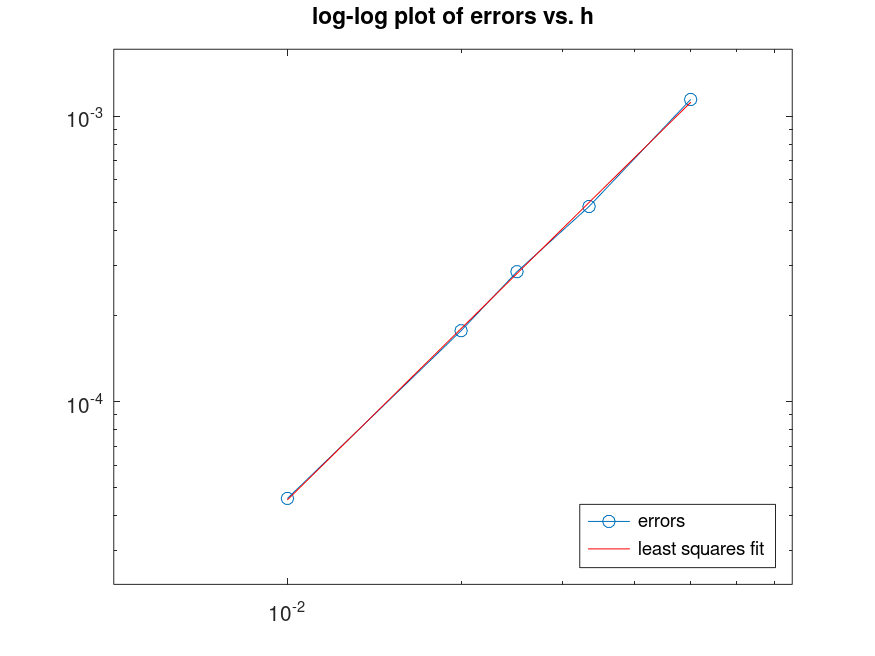
\includegraphics[width=\textwidth]{problem_2b_heatTRBDF2_error.png}
            \caption{TR-BDF2 error}
        \end{subfigure}
        \caption[]{TR-BDF2 solution}
    \end{figure*}

    The least squares fit from above corresponds to $h$ versus error, and because \linebreak
    $\Delta t = k = 4h = 4 \Delta x$, we see that the  method is indeed \linebreak
    $\mathcal{O}\left(h^2 + k^2\right)$, as desired.
    \ \\
\end{solution}